\justifying
\NSFCBodyText

\subsubsection{研究背景与意义}

新疆山地与盆地相间，天山南北坡和两大盆地的高程、下垫面及地形遮蔽差异，使近地面气温、风场、短波辐射和降水呈现不同的空间组织。区域气候影响研究需要同时认识这些变量的局地变化及共同出现的条件。例如，同一网格平均辐射条件下，山坡与盆地的温度和风环境仍可能明显不同。将粗网格值直接赋给整个区域，会掩盖这种差异，并影响对资源、生态和极端气象条件的综合判断。本项目围绕气象场本身的高分辨率增强开展研究，为包括新能源资源分析在内的下游应用提供基础资料。

清华大学联合地球系统模式（Community Integrated Earth System Model，CIESM）为研究气候系统及其变化提供了数值模拟基础。其模式发展与历史试验已形成公开成果，同时仍存在需要识别和处理的系统偏差\cite{Lin2020CIESM}。第六次国际耦合模式比较计划（CMIP6）的共同试验和资料标准，为追溯试验、成员、变量及版本提供了条件\cite{Eyring2016CMIP6}。对于区域应用，模式能够提供的大尺度气候状态与复杂地形下所需的局地气象信息之间仍有尺度差距。通过提高全球模式分辨率直接弥合差距需要增加计算成本；利用公开参考资料学习条件细节，为既有模式输出提供区域增强，是本课题拟探索的路径。

这里的高分辨率增强具有两个相互关联的要求：一是恢复具有地形差异和变量联系的亚网格结构，二是使重建场在重新聚合后仍与明确选定的大尺度状态相容。若只追求图像纹理清晰，生成的细节可能脱离模式提供的信息；若只匹配每个变量的均值，又可能损害温度、风、辐射和降水的共同变化。本项目以新疆典型山地和盆地为对象，研究这两项要求的兼容条件，并将方法组织为能够接入 CIESM 数据处理流程的算法模块。
% NSFC-ILLUSTRATED BEGIN F01
如图~\ref{fig:background} 所示，复杂地形下的跨尺度重建问题。网格为结构示意，虚线表示增强场向选定大尺度状态的回聚合检查。。
\begin{figure}[htbp]
\centering
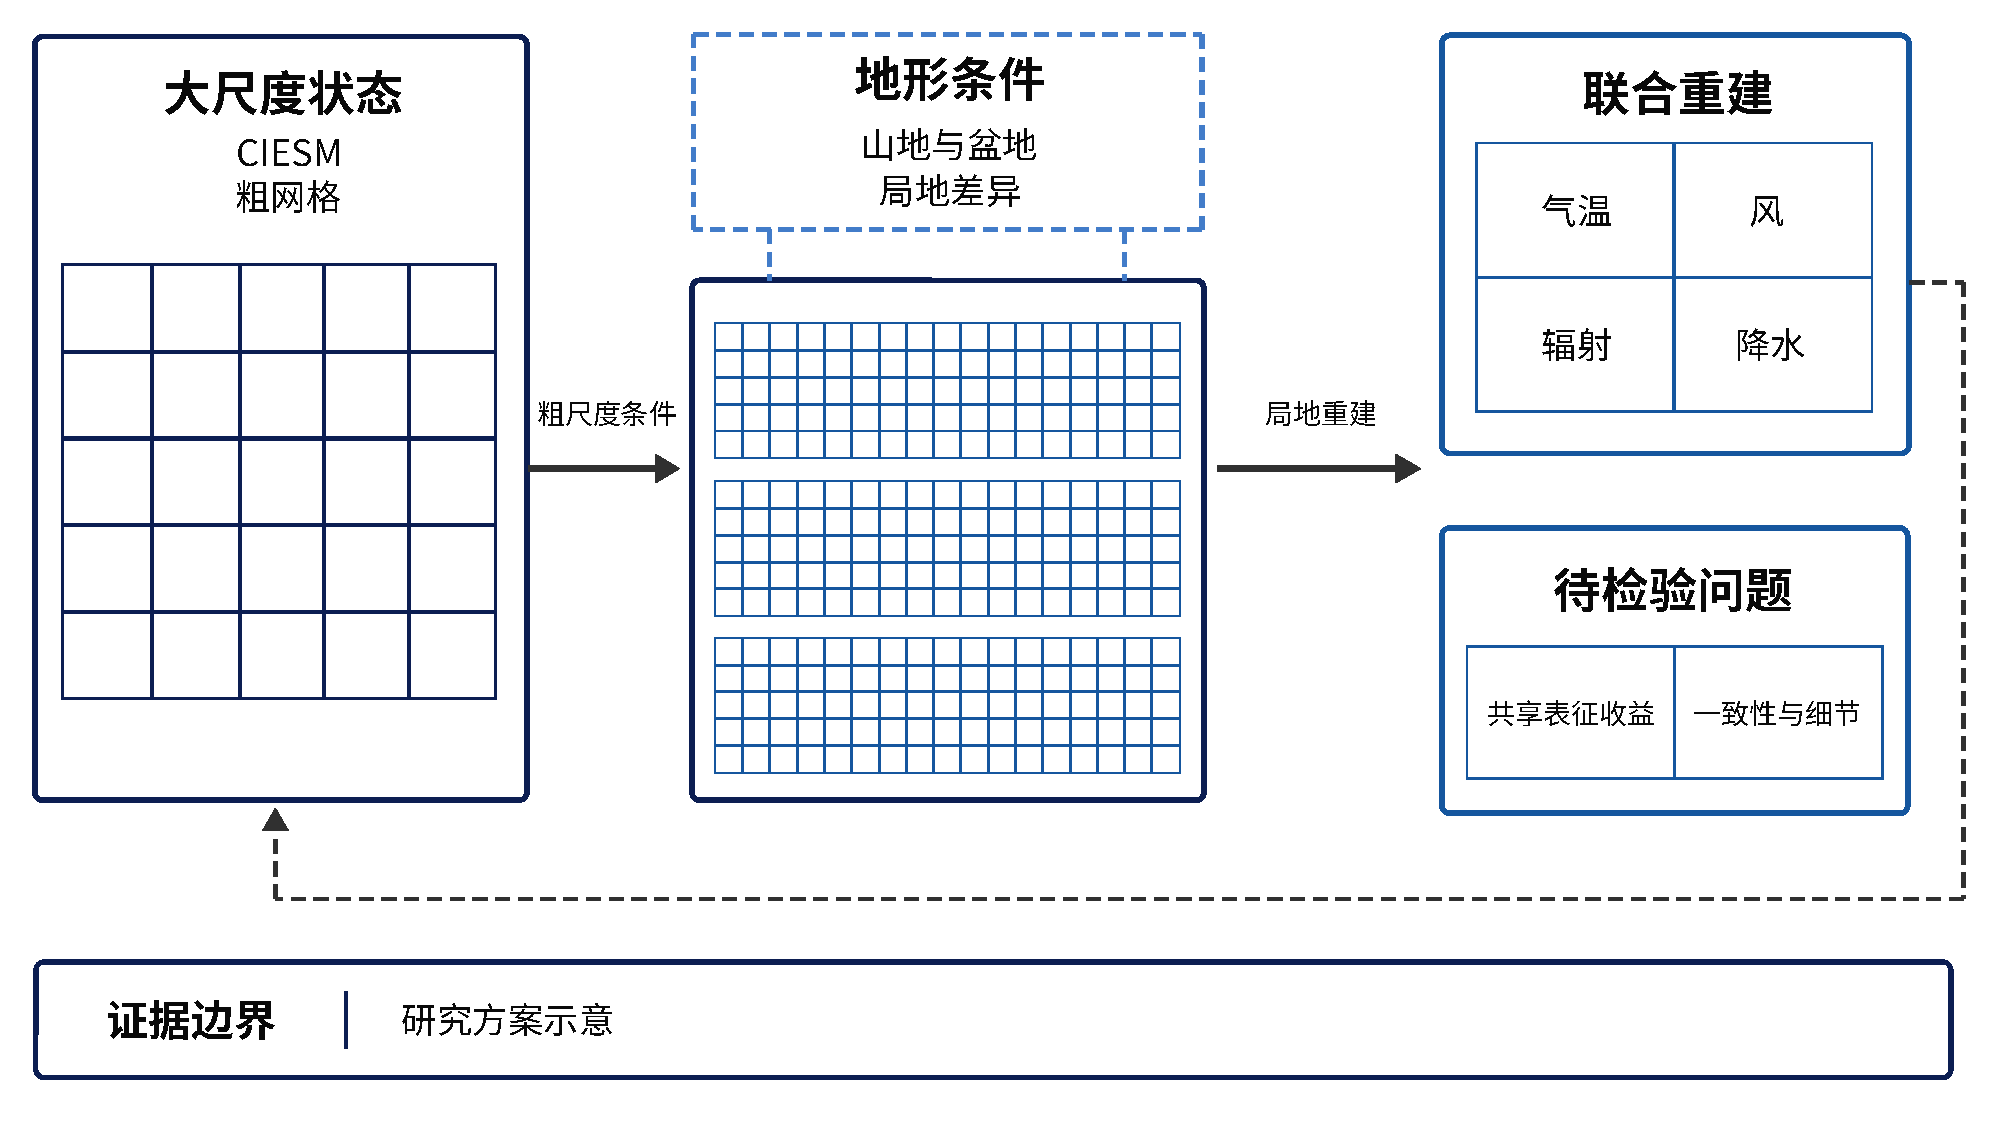
\includegraphics[width=0.95\linewidth]{figures/F01-background.pdf}
\caption{复杂地形下的跨尺度重建问题。网格为结构示意，虚线表示增强场向选定大尺度状态的回聚合检查。}
\label{fig:background}
\end{figure}
% NSFC-ILLUSTRATED END F01


本课题的研究期限为 2027 年一年，拟申请 P02“算法或数据集”方向，申请经费建议额为 4.5 万元。研究重点放在可复现的数据增强方法、约束效应及接口应用验证。拟通过限定变量、区域和实验层次，形成与课题周期和资源相匹配的证据，而不预先假定增加网格数量必然增加真实气象信息。

\subsubsection{国内外研究现状及发展动态分析}

\textbf{（1）参考资料与跨尺度对应关系。}
欧洲中期天气预报中心第五代再分析（ERA5）利用数值模式和观测同化提供连续再分析资料，是构造时空样本的重要来源\cite{Hersbach2020ERA5}。

ERA5 陆面再分析（ERA5-Land）采用更细的陆面网格，并由 ERA5 大气强迫驱动；其网格尺度和陆面模拟的改进，为地形相关研究提供了补充，但二者并非独立证据\cite{Munoz2021ERA5Land}。尤其对于近地面风、辐射和降水，必须逐变量检查原始强迫、插值与修正方式，不能仅依据标称网格大小认定细节更真实。

建立训练样本还需区分天气预报与自由运行气候模拟。后者即使覆盖同一历史年份，也不意味着与再分析资料逐日出现相同的天气过程。DeepESD 等研究以再分析建立大尺度预测因子与区域气候变量的关系，再将关系用于气候模式，体现了统计降尺度中 perfect-prognosis 的基本思路\cite{Bano2022DeepESD}。这一思路能避免直接以原始气候模拟和观测日期拼接成监督样本，但仍依赖预测因子的分布适应性与训练关系的稳定性。

\textbf{（2）从空间纹理到多变量时空重建。}
DeepSD 将卷积超分辨率引入气候资料增强，为从粗网格推断细网格提供了较早的实现路径\cite{DeepSD2017}。Stengel 等对风和太阳辐射开展对抗式超分辨率研究，显示了面向资源评估的应用潜力\cite{Stengel2020}。Serifi 等进一步比较不同气候变量的空间、时间重建，指出数据类型和采样频率会影响适宜的网络结构\cite{Serifi2021}。这些结果提示，温度等较平滑变量与间歇性降水不宜共享完全相同的误差模型。

近年来，生成模型开始描述给定粗尺度条件下可能出现的细尺度分布。Harris 等在降水随机降尺度中结合概率评分、空间谱和校准诊断评价生成结果\cite{Harris2022}。CorrDiff 将条件均值与随机残差分开建模，用于公里尺度大气场降尺度\cite{Mardani2025CorrDiff}。Schmidt 等已研究多变量、时空连续的条件生成轨迹\cite{Schmidt2025Coherent}。因此，本项目不能将“使用生成模型”或“联合多个变量”本身作为创新依据，需通过可对照实验说明地形条件和约束在特定资料条件下带来了什么增量。

\textbf{（3）偏差校正、变量依赖与非配对迁移。}
传统单变量分位数校正能够调整边缘分布，但变量间和空间上的依赖需要单独评估。Cannon 提出的多变量分位数映射为联合分布校正提供了参照\cite{Cannon2018MBCn}；Lange 的 ISIMIP3BASD 将趋势保持、偏差校正和统计降尺度的职责加以区分\cite{Lange2019ISIMIP}。Wang 与 Tian 已将深度超分辨率和趋势保持校正结合，用于多变量气候场\cite{Trend2024}。这些近邻研究意味着，本项目应把强统计方法纳入比较，并报告校正原始模式状态所产生的变化。

对非配对资料，Bischoff 与 Deck 研究了地球流体场的扩散桥变换\cite{Bischoff2024Unpaired}，Wan 等提出先粗尺度去偏、再条件采样的框架\cite{Wan2023}。Hess 等研究了尺度适应与未知气候条件下的高效生成降尺度\cite{Hess2025Scale}。Aich 等通过共享表示处理 地球系统模式降水的偏差校正和降尺度，表明无需把原始模式轨迹与观测轨迹强行配对，也能构造监督学习所需的对应关系\cite{Aich2026Diffusion}。然而，非配对方法仍需明确哪些尺度被保留、哪些统计量被调整，以及该选择是否适合目标区域。

\textbf{（4）物理一致性与泛化评价。}
Geiss 等将显式聚合约束用于大气化学场重建，并考虑网格面积差异\cite{Geiss2022}；González-Abad 等研究了温度变量之间的硬约束\cite{Gonzalez2024Hard}。相关工作说明，能够明确写成数学条件的约束可以嵌入模型输出；其适用性取决于变量定义和观测支持。只包含温度、近地面风、地表短波辐射及降水的资料，并不足以闭合完整水量和能量收支。

偏差校正的过程合理性、极端外推和区域迁移，是检验这些方法的关键。Maraun 等强调从物理过程理解校正的适用边界\cite{Maraun2017}；Rampal 等专门比较较暖气候条件下的降水极端外推\cite{Rampal2024}；近期区域预训练研究考察了不同参考数据集之间的适应性\cite{Pretrain2026}。据此，评价不能停留在随机划分样本上的平均误差，还应检验连续时段、不同地形及训练域以外区域的表现。

\subsubsection{现有研究的不足}

现有成果已覆盖本项目拟采用的多项技术，但在新疆 CIESM 数据增强这一具体对象上，仍需回答以下问题。

第一，粗细资料的对应关系尚需逐变量建立。再分析资料内部的人工降质样本可提供配对真值，却未必覆盖真实 CIESM 的偏差；将模型用于 CIESM 后获得的分布改善，也不能直接证明每一天气过程被正确恢复。两类实验之间需要明确的解释边界。

第二，地形条件与变量联合的独立贡献尚需辨别。增加辅助信息、扩大网络容量和加入约束都可能改善评价指标，若同时改变，难以判断收益来自哪一因素。需要在相同数据、参数量级和计算预算下，区分多变量共享、地形先验及显式一致性条件的作用，并检查降水等变量是否因联合训练受到负迁移。

第三，一致性约束与有效细节之间可能存在权衡。与未经校正的 CIESM 强制一致，可能保留其系统偏差；与校正后的场一致，则必须报告校正对模式信号的影响。经验性的温度垂直梯度、变量相关性及空间梯度也会随季节和天气型变化，不宜作为普适物理定律硬性施加。约束是否改善独立验证，须由对照结果而非约束名称判定。

\subsubsection{关键科学问题与研究切入点}

本项目拟回答的中心问题是：\textbf{在 CIESM 与参考资料存在分布差异的条件下，复杂地形信息与多变量依赖能否提供稳定的亚网格重建增益，并与可定义的大尺度一致性条件兼容？}

这一问题包含三个子问题：粗尺度状态经适当校正后，哪些空间和时间结构具有可学习、可迁移的条件关系？地形信息能否使变量间的信息共享在山区与盆地均产生增益，其失效条件是什么？将显式聚合条件与经验约束分开后，如何识别限制非物理输出与过度压平局地变化之间的界限？

据此提出可证伪假设：在固定资料、偏差校正和模型容量条件下，地形条件下的共享表征有望降低有限样本估计误差，进而减少复杂地形单元的条件重建误差，并改善跨变量共同变化的统计特征；加入适当的聚合与变量定义约束，有望在保持这些增益的同时降低不一致残差。将增益定义为基线误差减去本方法误差。若增益区间上界低于预设最小有意义增益，则不支持相应的有效增益假设；下界高于该阈值且各变量非退化条件均通过时，才判为支持；其余情况报告证据不足。地形与共享的交互不成立时，撤回地形增强作用的解释。

研究将先建立可追溯的训练与验证资料，再构建联合重建模型，通过单变量、无地形和不同约束强度的对照确定增益来源，最后在 CIESM 数据上完成分布、结构及接口应用验证。预期形成的科学认识是地形、变量依赖和尺度条件共同作用的适用边界；预期形成的方法成果是具有可检查输入输出关系的 CIESM 区域气象场增强模块。
